\documentclass[25pt, a0paper, portrait, margin=0mm, innermargin=15mm, blockverticalspace=12mm, colspace=15mm, subcolspace=8mm]{tikzposter}
\usepackage{amsmath,amssymb,graphicx,booktabs}
\graphicspath{{../figures/}}
\usetheme{Simple}
\usecolorstyle{Denmark}
\newcommand{\Mpch}{\,h^{-1}\mathrm{Mpc}}

\title{\parbox{0.9\linewidth}{\centering ASTRA environment-split clustering:\\[0.3em] cosmological forecasts with emulators and comparison with density split}}
\author{Hugo Nguyen}
\institute{DESI}

\begin{document}
\maketitle

\begin{columns}
% ---------------------------------------------------------------- column 1
\column{0.33}
\block{Why environments?}{
The two-point correlation function (2PCF) captures all the information of a Gaussian field, but the late-time Universe is not Gaussian: matter collapses into halos, filaments and nodes, and empties voids. \textbf{Environment statistics} recover part of the missing information by measuring clustering separately in dense and empty regions.

\vspace{0.5em}
\textbf{Goal:} quantify how much \textbf{ASTRA} environment statistics improve constraints on $\omega_b$, $\omega_{\rm cdm}$, $n_s$, $\sigma_8$, $w_0$, $w_a$ over the 2PCF, and compare with \textbf{density split}, the reference method.
}

\block{Two ways to define an environment}{
\textbf{ASTRA:} Delaunay tessellation of galaxies + random points; each point gets
$$r=\frac{N_{\rm gal}-N_{\rm rand}}{N_{\rm gal}+N_{\rm rand}}$$
from its neighbours. No smoothing scale: adaptive, local.

\textbf{Density split:} galaxy density smoothed on $10\Mpch$.

Points are ranked into quartiles Q1 (voids) to Q4 (clusters), or into ASTRA classes (void, sheet, filament, knot).

\vspace{0.5em}
\begin{tikzfigure}
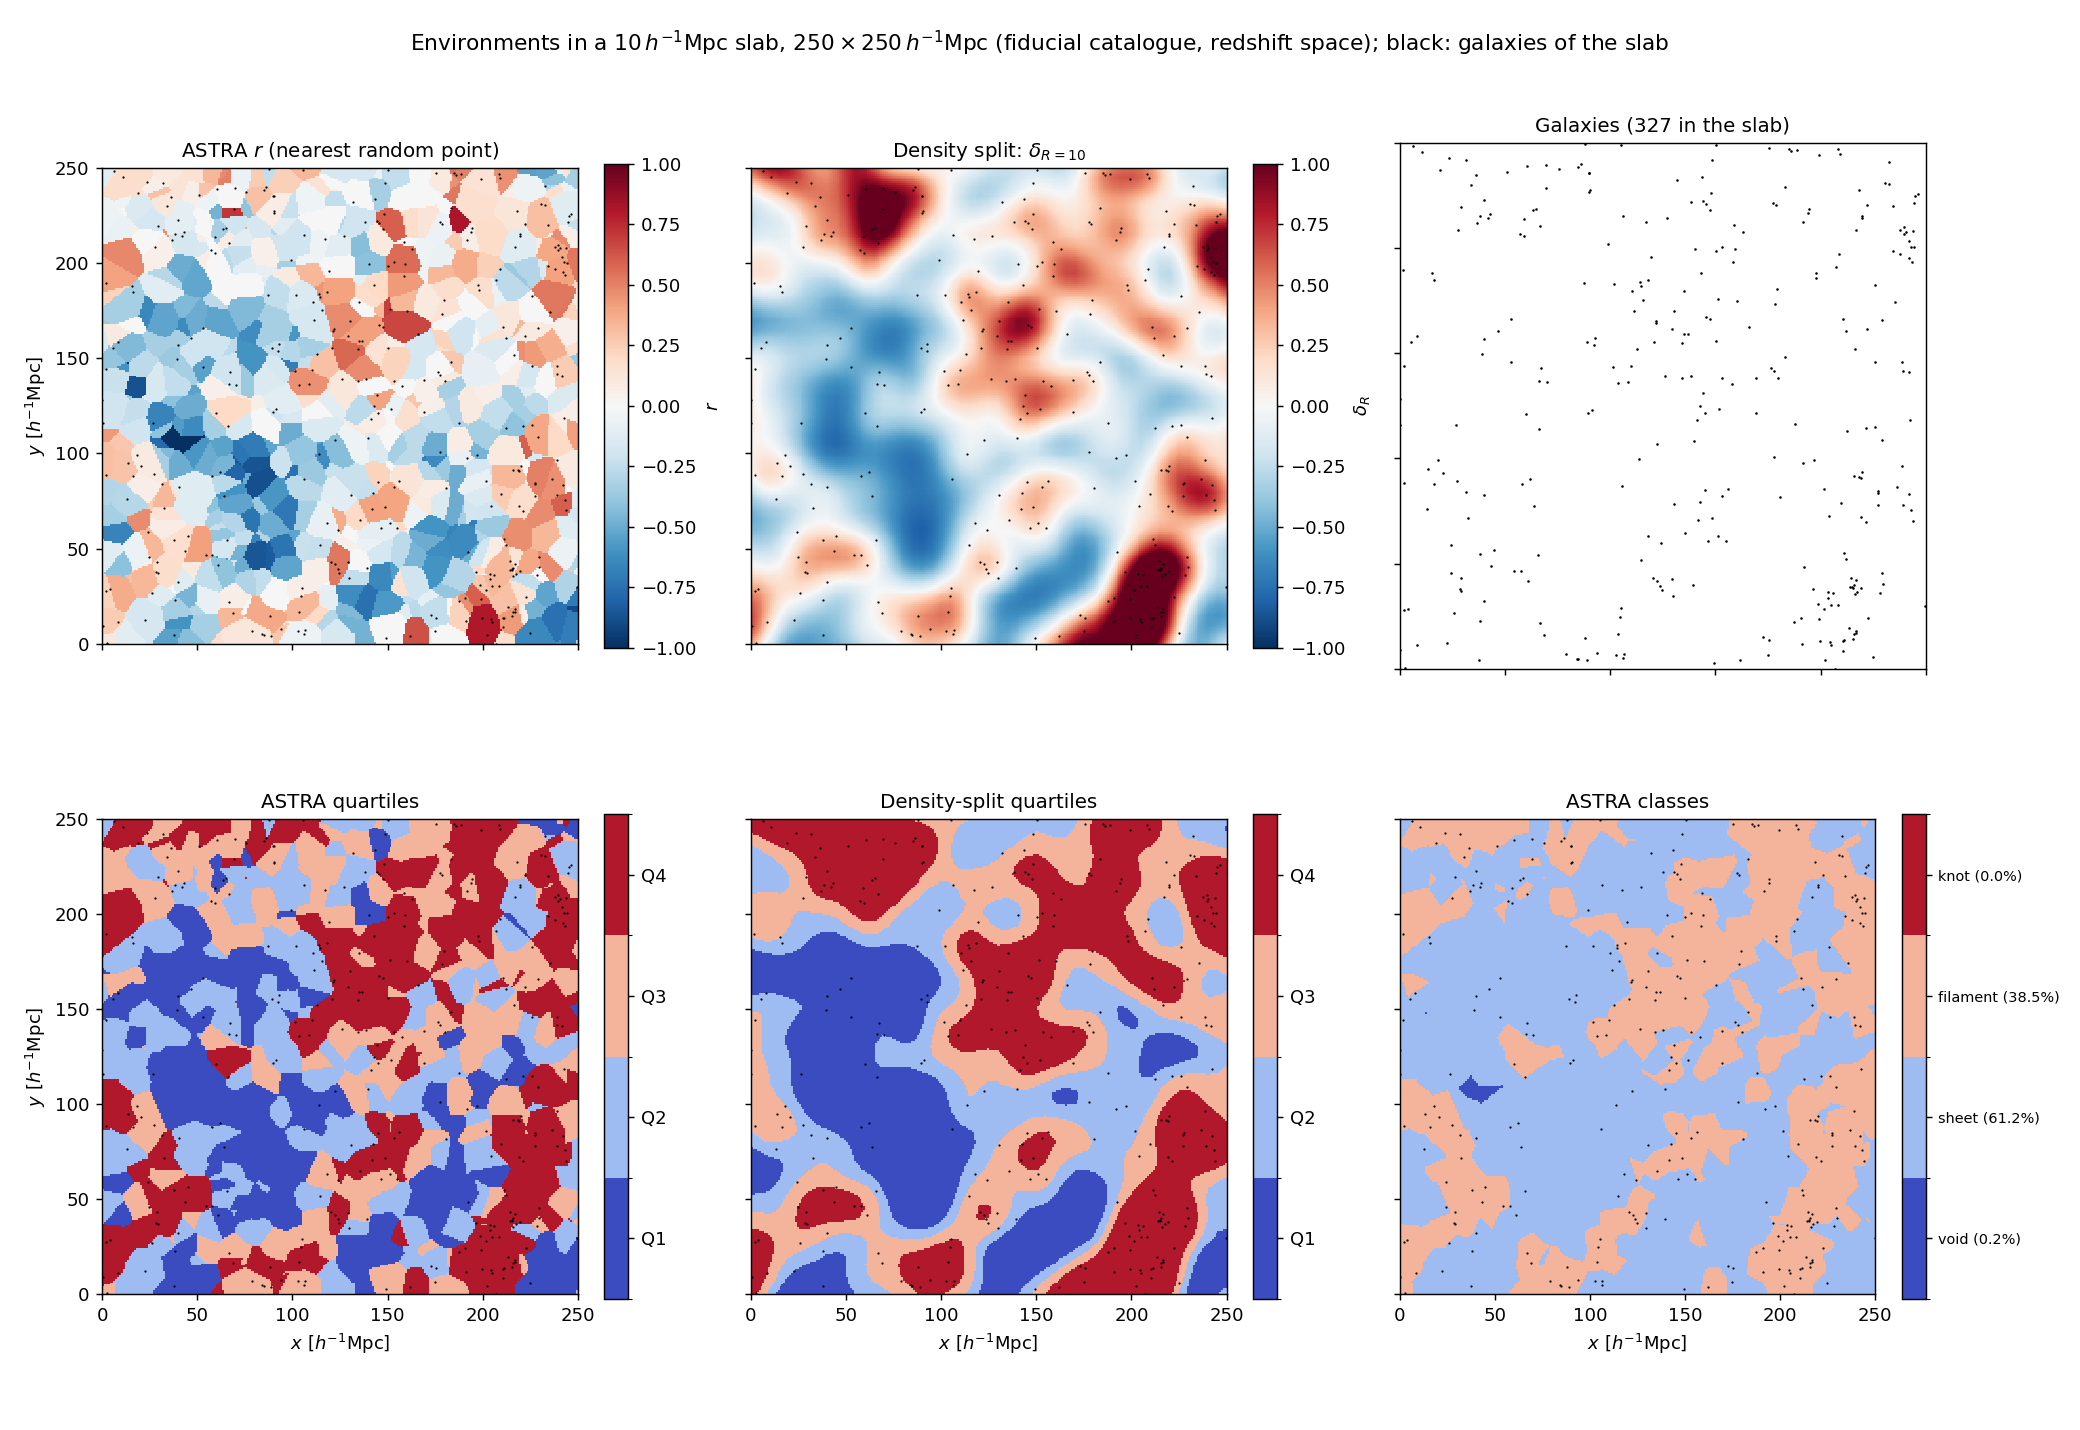
\includegraphics[width=0.98\linewidth]{env_maps.png}
\end{tikzfigure}
{\small Environments in a $250\times250\times10\Mpch$ slab; black dots: galaxies.}
}

\block{Data and method}{
\begin{tabular}{p{0.3\linewidth}p{0.62\linewidth}}
\textbf{AbacusSummit} & DESI-like LRG mocks, 85 cosmologies: measurements, emulator \\
\textbf{DESI official mocks} & 1786 independent boxes: covariance \\
\textbf{Quijote} & 500 paired simulations per parameter: clean derivatives \\
\end{tabular}

\vspace{0.5em}
Auto- and cross-correlations of the quartiles (monopole + quadrupole) $\to$ covariance + derivatives $\to$ \textbf{Fisher forecasts}. A \textbf{neural-network emulator} of all the statistics gives derivatives at fixed galaxy--halo connection, and an \textbf{MCMC} tests the full inference.
}

\block{Emulator accuracy}{
\begin{tikzfigure}
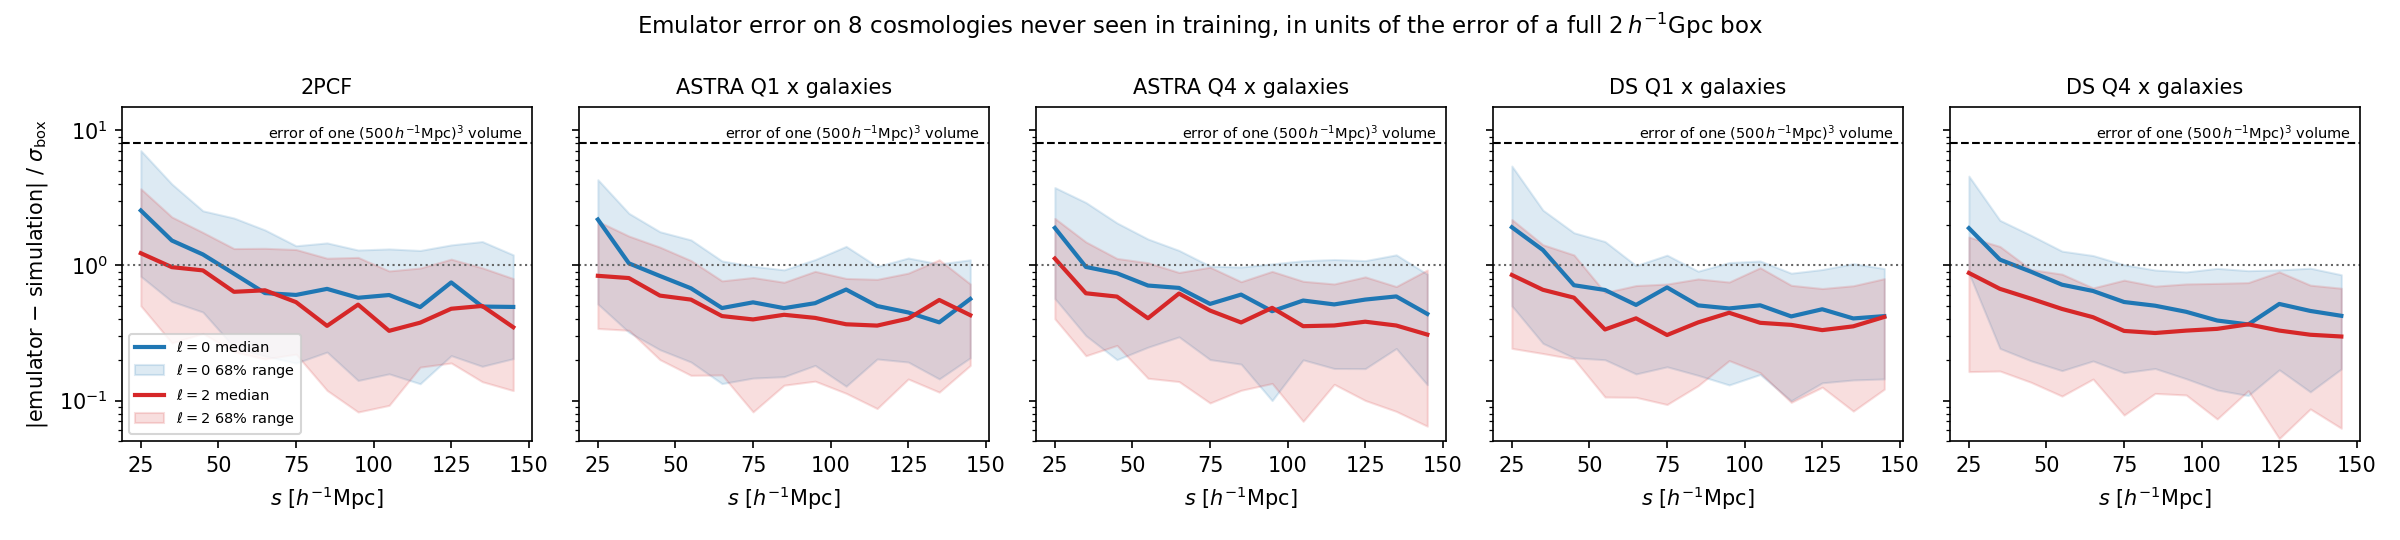
\includegraphics[width=\linewidth]{readable_emulator_validation.png}
\end{tikzfigure}
{\small Error on 8 cosmologies never seen in training: $\sim0.5\sigma$ of a $2\,h^{-1}$Gpc box, ten times below the error of the volume used for the forecasts (dashed).}
}

% ---------------------------------------------------------------- column 2
\column{0.34}
\block{Clustering by environment}{
\begin{tikzfigure}
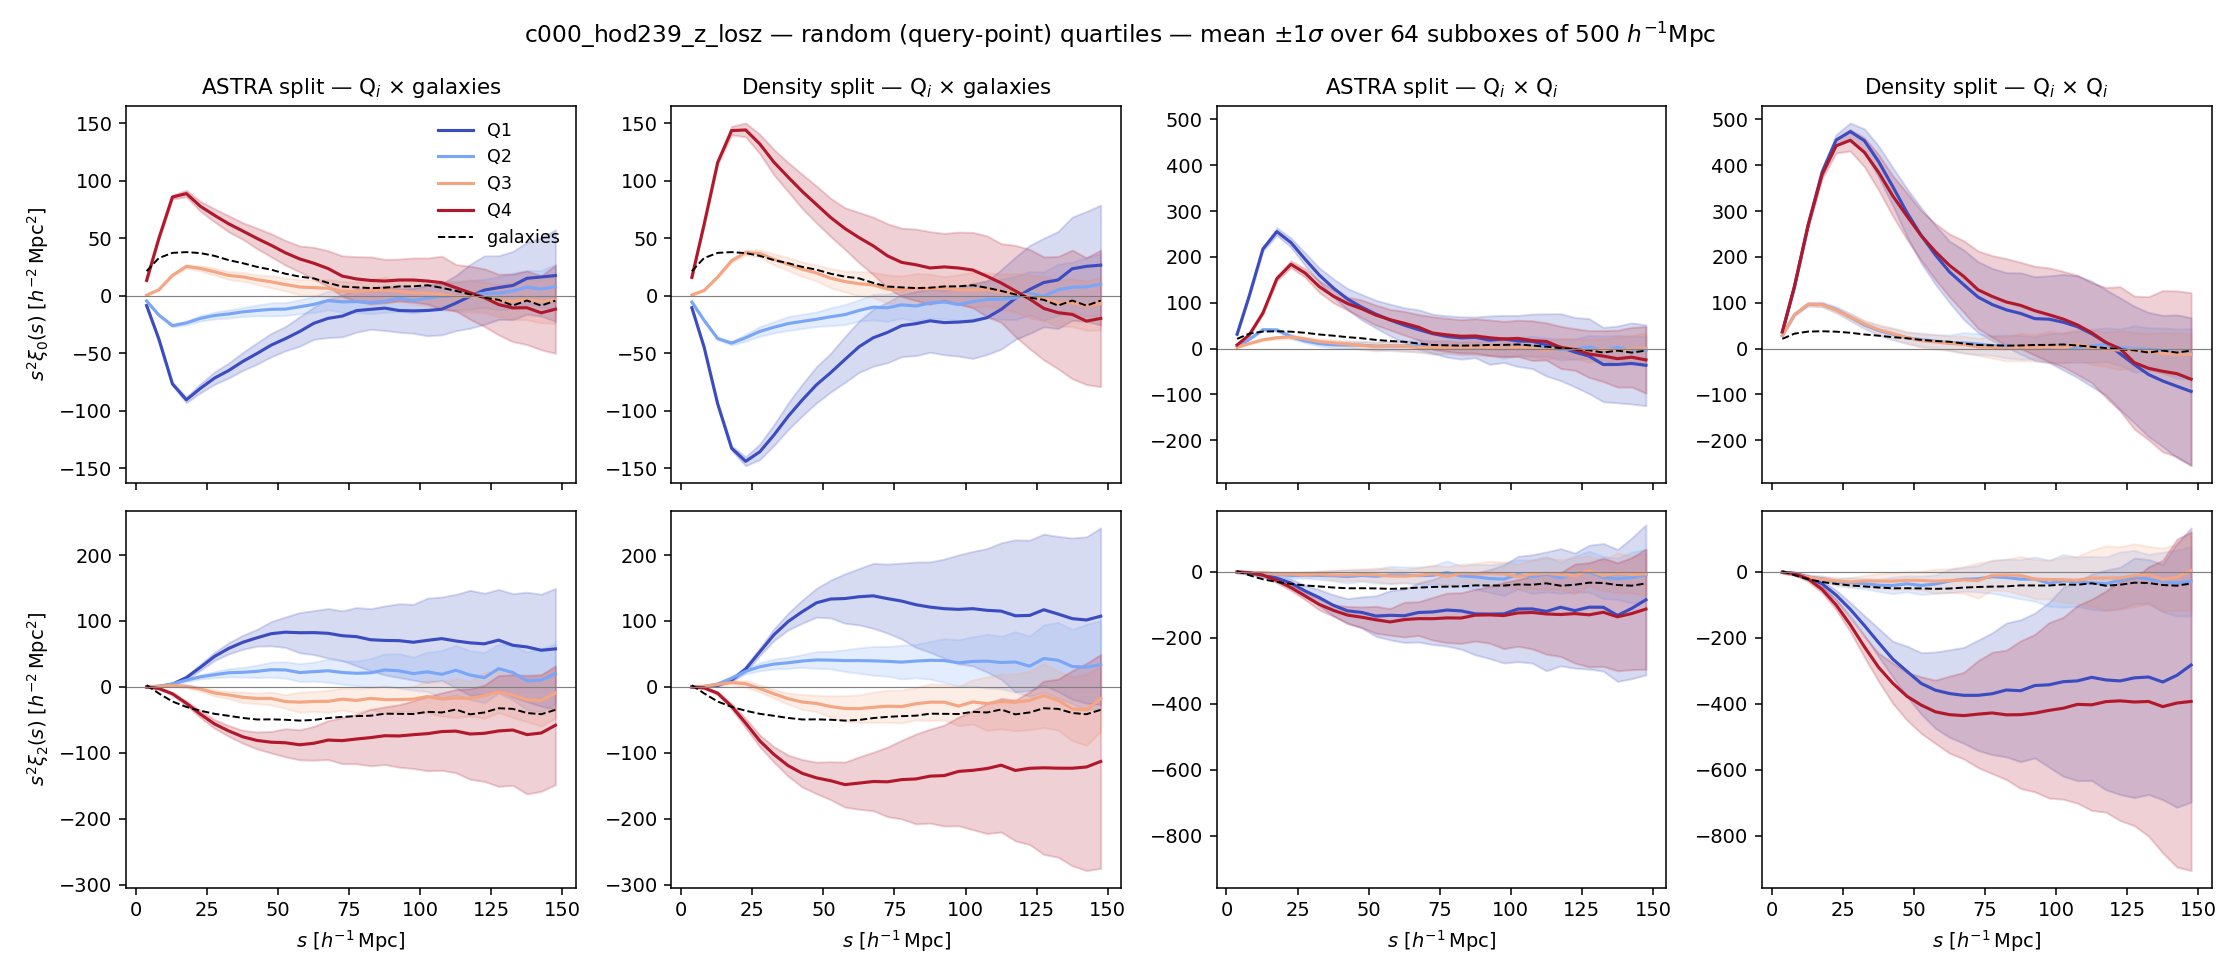
\includegraphics[width=\linewidth]{v2_multipoles_rand.png}
\end{tikzfigure}
{\small Monopole (top) and quadrupole (bottom) of the random-quartile cross- and auto-correlations. ASTRA signals are $\sim1.6\times$ weaker, but information is about signal \emph{and} noise.}
}

\block{Gain over the 2PCF}{
\begin{tikzfigure}
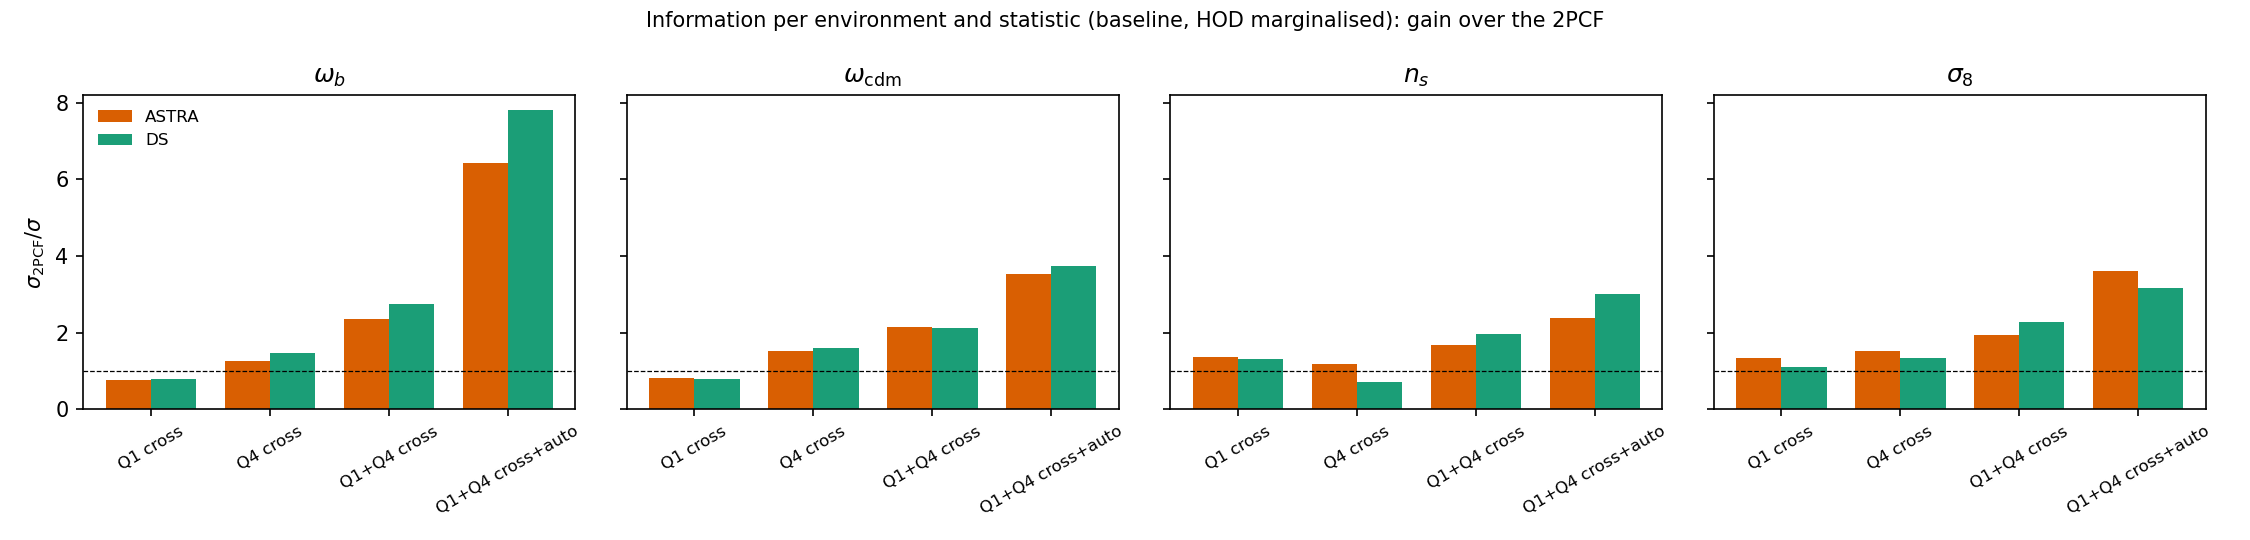
\includegraphics[width=\linewidth]{v2_quartiles.png}
\end{tikzfigure}
{\small $\sigma_{\rm 2PCF}/\sigma$ per environment and statistic. Each quartile alone is about as informative as the 2PCF; combined, and with auto-correlations, they are several times better.}

\vspace{0.4em}
\begin{center}
\begin{tabular}{lcc}
\toprule
 & vs 2PCF & DS / ASTRA \\
\midrule
gain on $\omega_b,\dots,w_a$ & $\times1.6$--$3.1$ & $0.8$--$1.1$ \\
ASTRA + DS combined & \multicolumn{2}{c}{further $\times1.2$--$2.4$} \\
\bottomrule
\end{tabular}
\end{center}
}

\block{Inference test (MCMC)}{
\begin{tikzfigure}
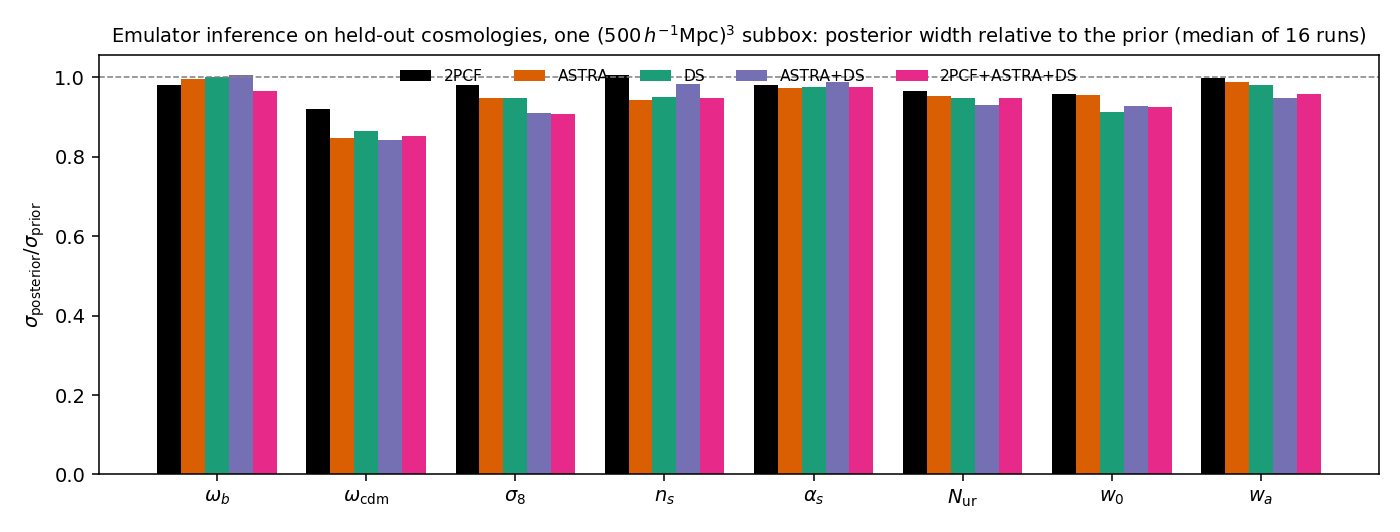
\includegraphics[width=\linewidth]{v2_mcmc_widths.png}
\end{tikzfigure}
{\small Posterior width / prior width on held-out cosmologies. The posteriors are unbiased and calibrated; one $(500\Mpch)^3$ volume is too small to discriminate the statistics, a full box is limited by the emulator error.}
}

\block{Fisher contours}{
\begin{tikzfigure}
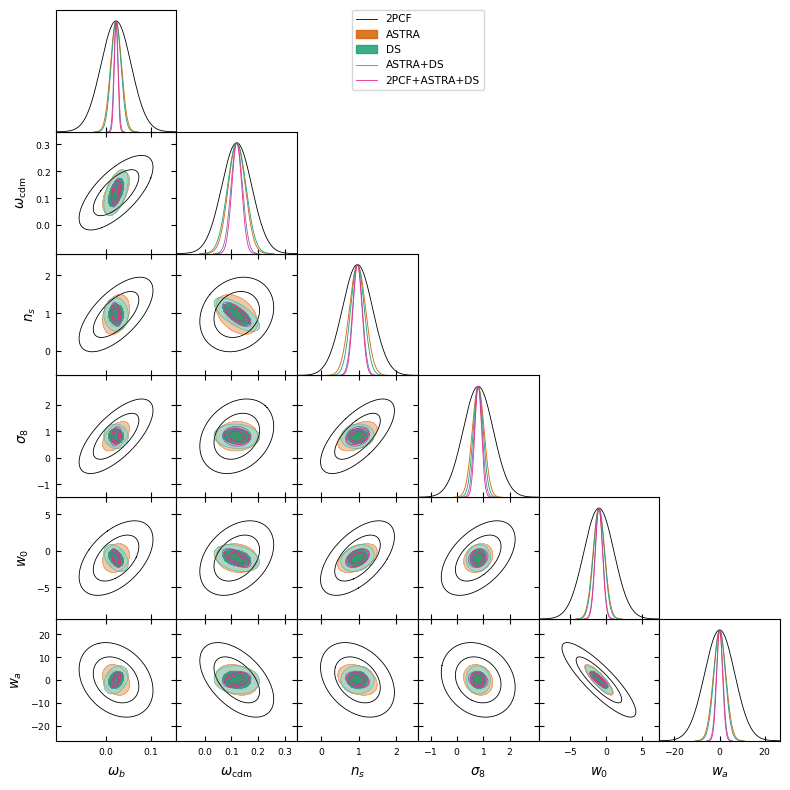
\includegraphics[width=0.9\linewidth]{v2_triangle.png}
\end{tikzfigure}
{\small 2PCF, ASTRA, density split and combinations, one $(500\Mpch)^3$ volume, galaxy--halo connection marginalised.}
}

% ---------------------------------------------------------------- column 3
\column{0.33}
\block{ASTRA cosmic-web classes}{
With fixed thresholds, voids and knots hold $<1\%$ of the points: two dominant classes (sheets, filaments). Yet on Quijote, their auto- and cross-correlations are the \textbf{most constraining statistic}:
\begin{tikzfigure}
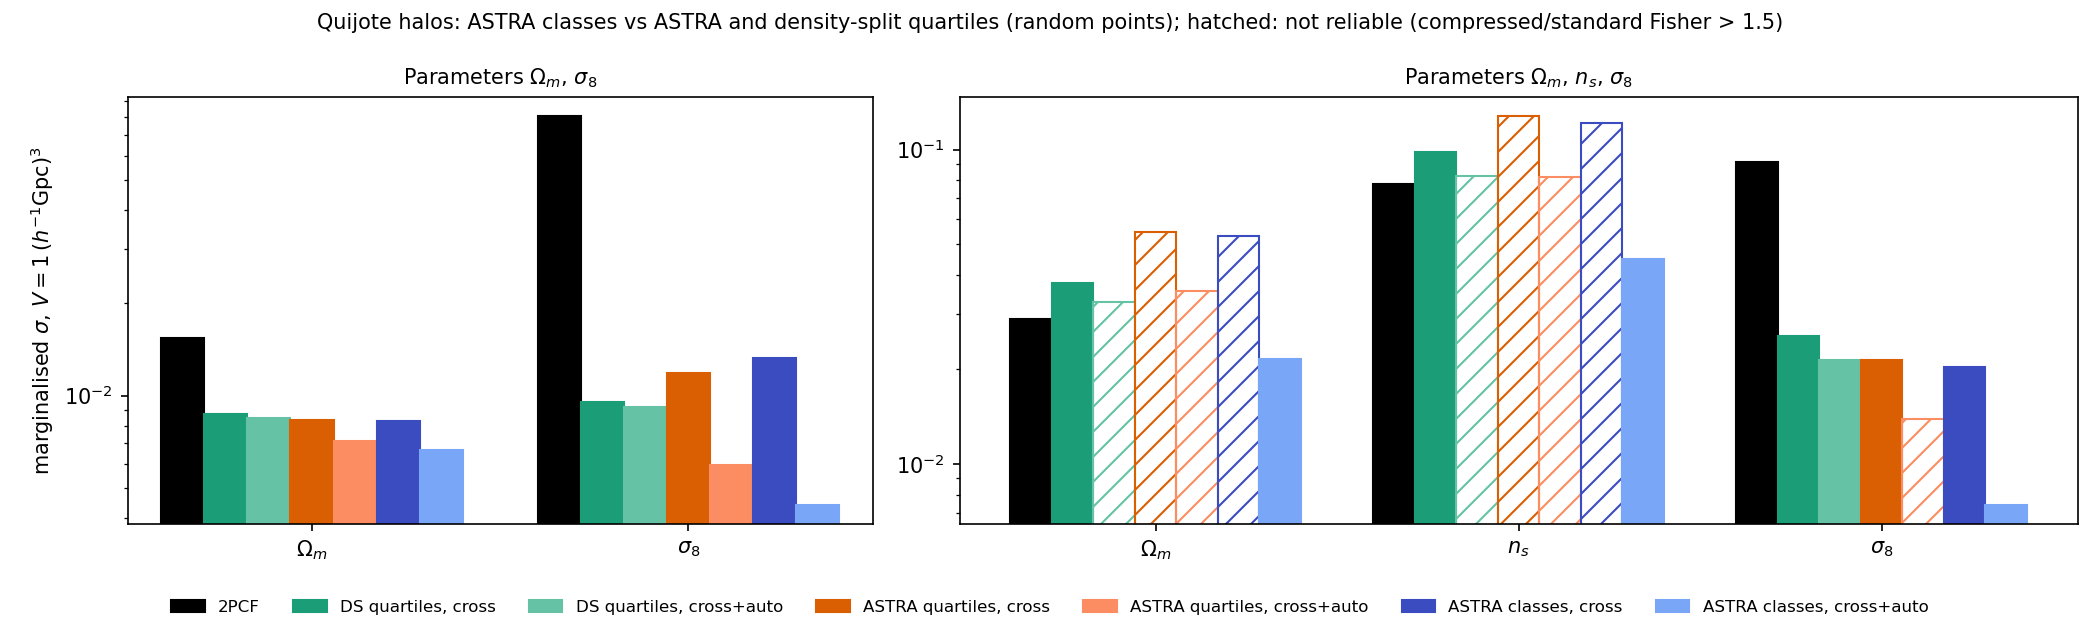
\includegraphics[width=\linewidth]{classes_fisher.png}
\end{tikzfigure}
{\small $\sigma_8$ is \textbf{2--3 times} better constrained than with density split, robustly across data compressions.}
\begin{tikzfigure}
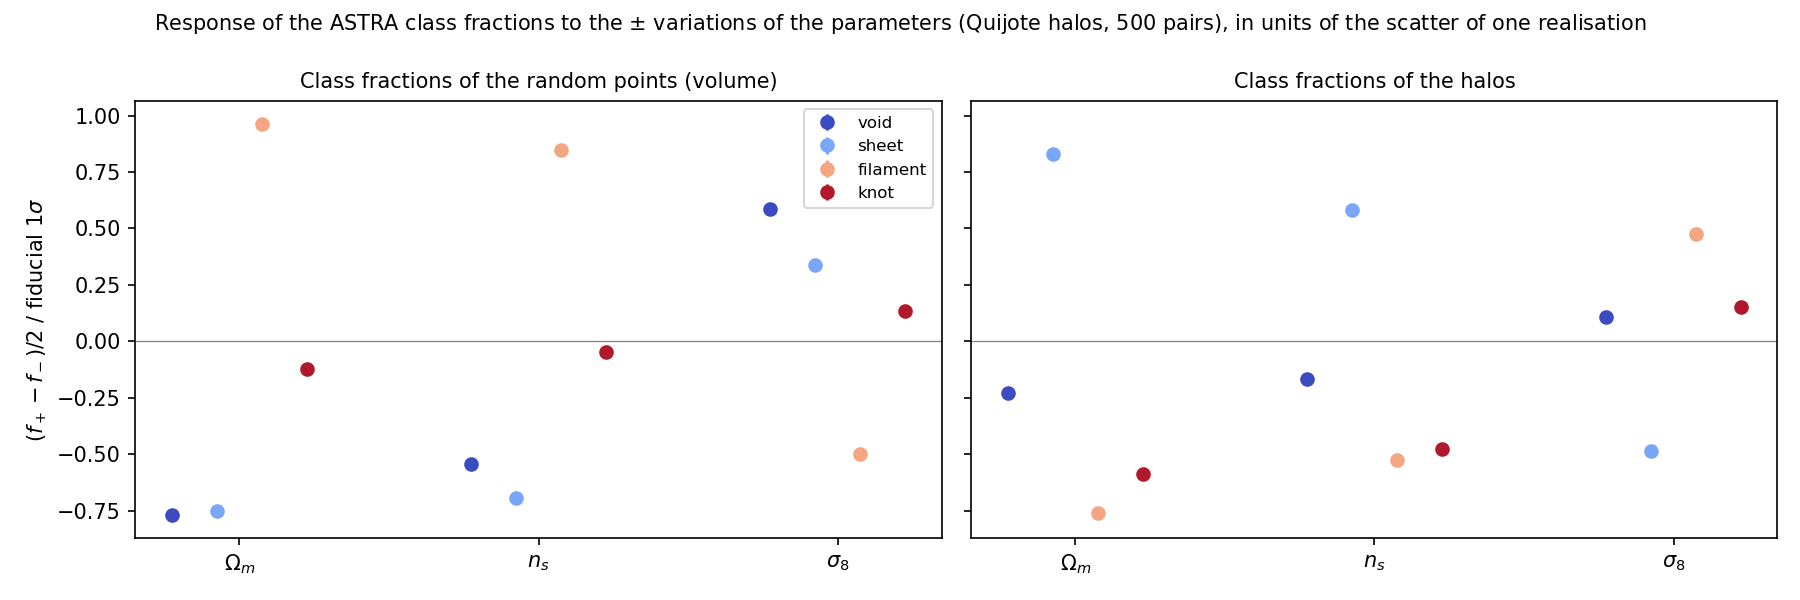
\includegraphics[width=\linewidth]{classes_response.png}
\end{tikzfigure}
{\small With fixed thresholds, the volume of each class responds to cosmology, which equal-size quartiles remove by construction.}
}

\block{What we learnt about the method}{
\begin{itemize}
\item Emulator suites draw a different galaxy--halo connection in each cosmology: finite differences measure it, not cosmology $\to$ emulator.
\item A covariance from one simulation box biased the comparison $\to$ 1786 independent boxes.
\item Derivatives of environment statistics of sparse tracers are noisy $\to$ two bracketing Fisher estimators identify reliable forecasts.
\item ASTRA adapts its scale to the density: model it at the density of the data.
\end{itemize}
}

\block{Conclusions}{
\begin{itemize}
\item ASTRA environment statistics constrain cosmology \textbf{$\sim2\times$ better than the 2PCF}.
\item As informative as density split, and \textbf{complementary}.
\item ASTRA \textbf{classes} constrain $\sigma_8$ 2--3$\times$ better than density split (Quijote).
\item Emulator + MCMC pipeline validated, ready for larger training sets.
\end{itemize}
\vspace{0.3em}
{\small Code: \texttt{github.com/Hugoooat/DESI\_astra} (branch \texttt{astra\_hugo\_v2})}
}
\end{columns}

\end{document}
